\chapter{uForth-Editor}
\label{chap:fortheditor}
In diesem Kapitel wird beschrieben, wie das Framework Xtext funktioniert und wie es verwendet wurde, um Features wie Syntax Highlighting, eine Outline und Dokumentations Popups für den Forth Editor zu implementieren.

\section{Xtext-Implementation des uForth-Editors}
Xtext ermöglicht es, das Grundgerüst einer Entwicklungsumgebung zu generieren. Dafür verwendet Xtext eine Extended Backus-Naur Form (EBNF) ähnliche Grammatik. Aus dieser Grammatik wird ein ANTLR-Parser und Klassen, die für den Editor benötigt werden, generiert. Um Xtext zu konfigurieren, wird die Dependency Injection (DI) Library Guice von Google verwendet. Mit Guice können viele Teile von Xtext in einem zentralen Modul mittels DI ersetzt werden.\\
Da Forth keinen monolithischen Compiler und somit keine statische Grammatik besitzt, kann keine Grammatik für Xtext geschrieben werden, die die gesamte Forth-Sprache beschreibt. Es wurde deshalb eine Xtext-Grammatik verwendet, die ungefähr der folgenden EBNF-Grammatik entspricht.

\begin{verbatim}
instructoin = create | function | word;
function = ':', identifier, { Word }, ';';
create = 'create', identifier, { literal ',' };
word = identifier;
\end{verbatim}

Die \verb!identifier!-Regel beschreibt alle gültigen Forth Identifier und die \verb!literal!-Regel alle gültigen Integer- und Double-Werte.
\\
Der daraus generierte Parser kann alle vom LCC generierten Forth Files parsen und reicht somit für die Entwicklungsumgebung aus. 

\newpage
\section{uForth Editor}
Der Editor unterstützt Syntax Highlighting für vordefinierte Forth-Wörter, Literals und Kommentare. Die Wörter werden in drei Gruppen unterteilt. Stack-Wörter, Memory-Wörter und arithmetischewörter. Alle Gruppen haben eine andere Farbe, die in der uForth Preference Page geändert werden kann. Die Abbildung \ref{fig:fortheditor} zeigt den uForth-Editor.


\begin{figure}[H]
	\centering
		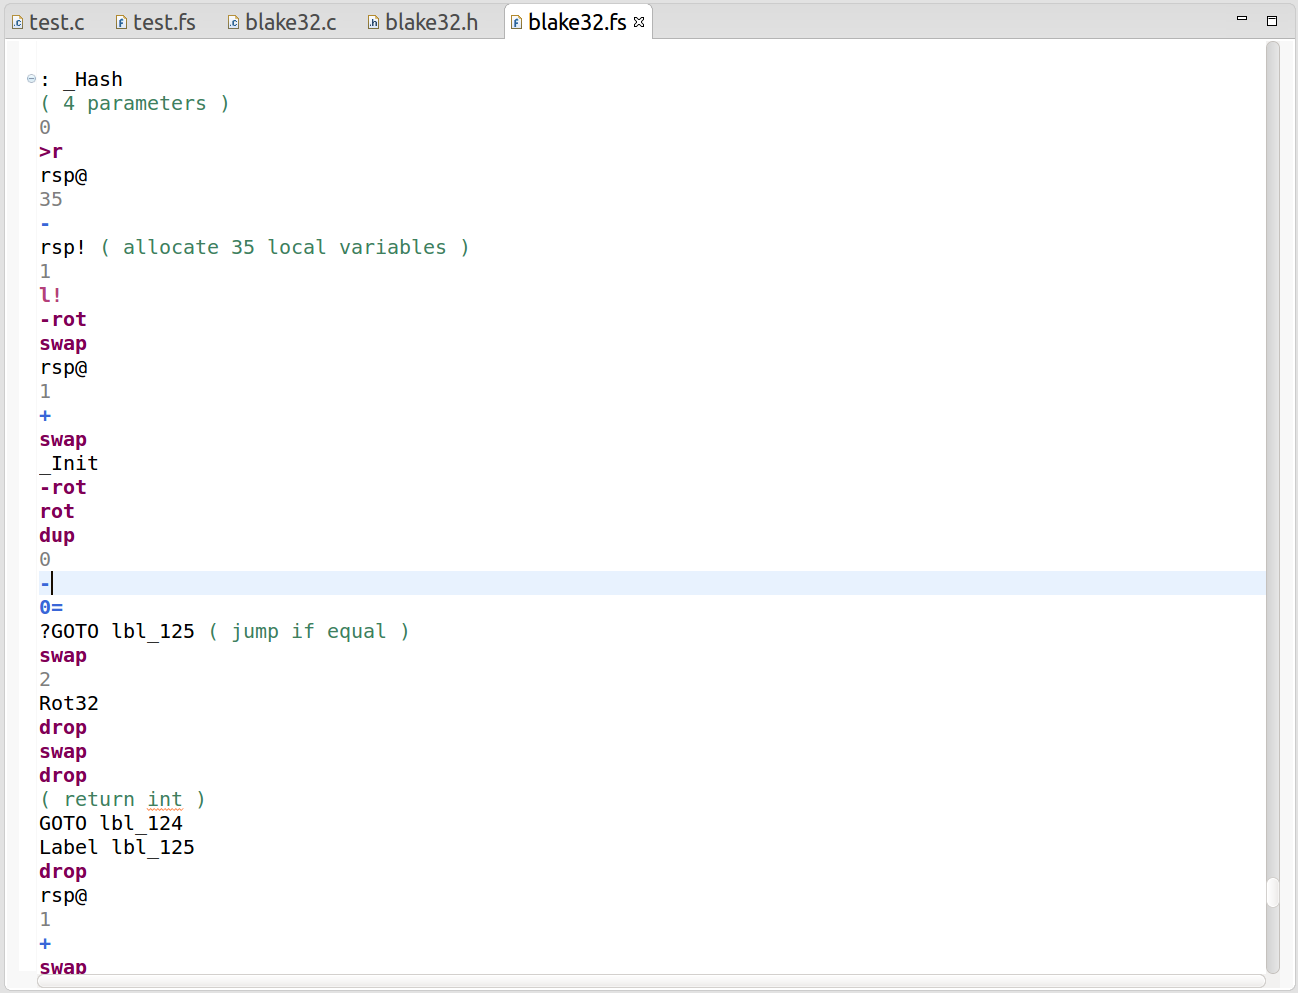
\includegraphics[scale=0.4]{fortheditor/fortheditor.png}
		\caption{uForth-Editor, der für den Debugger verwendet wird.}
		\captionsetup{margin=0cm,font={footnotesize}}
		\label{fig:fortheditor}
\end{figure}

\newpage

\subsection{Dokumentation der uForth-spezifischen Wörter}
Eine Dokumentation wurde für uForth-spezifischen Wörter, als Popup im Editor implementiert. Die Dokumentation wird dafür aus einer Textdatei gelesen. Die Abbildung \ref{fig:docpopup} zeigt eine Popup-Dokumentation zm Wort \verb!label!.

\begin{figure}[H]
	\centering
		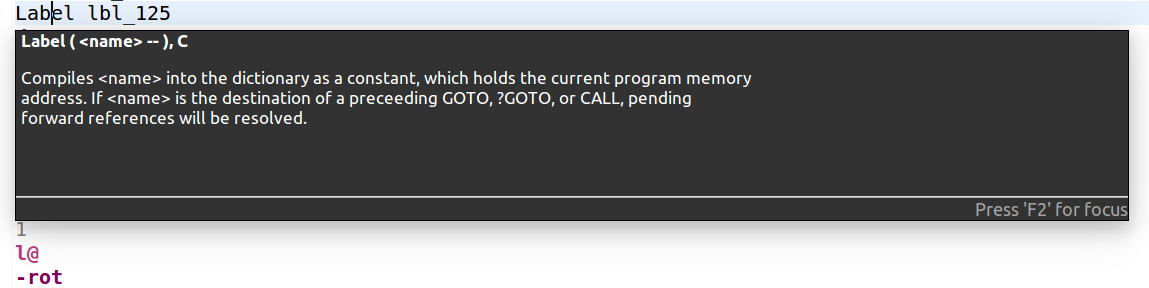
\includegraphics[scale=0.4]{fortheditor/doc.png}
		\caption{Popup Dokumentation zum Wort label. Die Dokumentation wird angezeigt, falls der Cursor sich über einem Wort befindet, für das eine Dokumentation verfügbar ist.}
		\captionsetup{margin=0cm,font={footnotesize}}
		\label{fig:docpopup}
\end{figure}

\subsection{Editor Outline}
Für den Editor steht zudem eine Outline zur Verfügung. Die Outline gliedert das Forth File nach den von der Grammatik spezifizierten Regeln. Für den uForth-Editor bedeutet das, dass das File nach Funktionen und Wörtern gegliedert wird.

\begin{figure}[H]
	\centering
		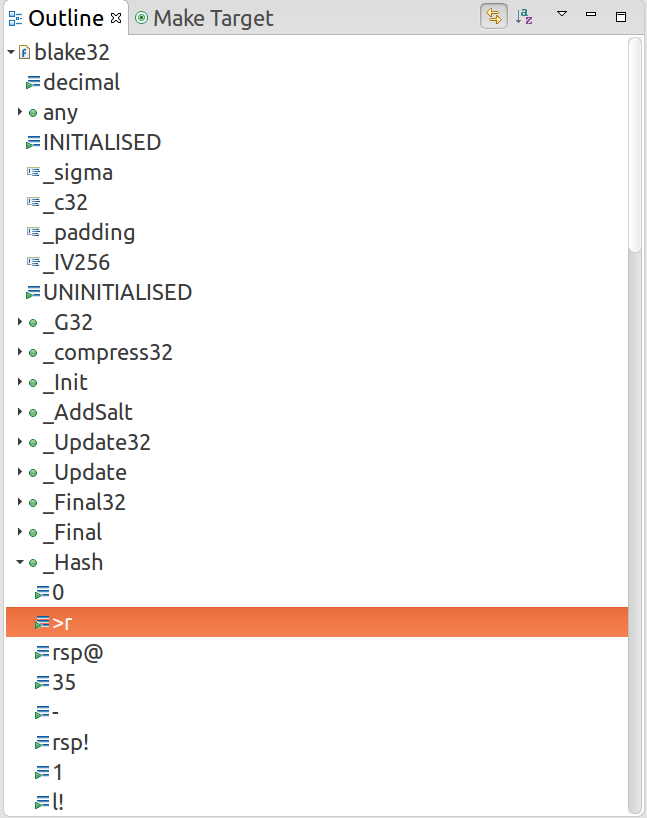
\includegraphics[scale=0.3]{fortheditor/outline.png}
		\caption{Outline zu einem Forth File. Die Outline gliedert das File in Funktionen und Wörter.}
		\captionsetup{margin=0cm,font={footnotesize}}
		\label{fig:outlineeditor}
\end{figure}

